\documentclass[crop,tikz,border=7pt]{standalone}

% math and formulas
\usepackage{amsmath}
\usepackage{amsfonts}
\usepackage{amssymb}
\usepackage[amssymb]{SIunits}
\usepackage{mathtools}
\usepackage{esvect} % for vector typesetting
\usepackage{bm} % for matrix typesetting
\usepackage{xfrac}

\usepackage{environ}


% ---Notation macros---

% math
\let\oldvec\vec
% \renewcommand{\vec}[1]{\bm{\mathbf{#1}}}
\renewcommand{\vec}[1]{\bm{#1}} % \bm vs \mathbf
\newcommand{\vecf}[1]{\bm{#1}} % \bm vs \mathbf
\newcommand{\vecelem}[1]{#1}
\newcommand{\vecarrow}[1]{\vv{#1}}
\newcommand{\mat}[1]{\bm{#1}}
\newcommand{\matelem}[1]{\mathit{#1}}
\newcommand{\ten}[1]{\mathbf{#1}}
\newcommand{\tenelem}[1]{\mathrm{#1}}
\newcommand{\set}[1]{\mathbb{#1}}

\newcommand{\trans}[1]{#1^{\mathsf{T}}}
\newcommand{\ifrac}[2]{\sfrac{#1}{#2}}
\newcommand{\deriv}[2]{\frac{\text{d}#1}{\text{d}#2}}
\newcommand{\partderiv}[2]{\frac{\partial #1}{\partial #2}}
\newcommand{\ideriv}[2]{\ifrac{\text{d}#1}{\text{d}#2}}
\newcommand{\ipartderiv}[2]{\ifrac{\partial #1}{\partial #2}}

\DeclarePairedDelimiter{\norm}{\lVert}{\rVert}

% machine learning
\newcommand{\param}{\lambda}


% misc
\newcommand{\keyword}[1]{\textbf{#1}}
\newcommand{\para}{\par\medskip}
\newcommand{\ds}{\displaystyle}

\newcommand{\keycode}[1]{\texttt{#1}}
\newcommand{\code}[1]{\texttt{#1}}


\let\oldcite\cite
\renewcommand{\cite}[1]{{\color{red}(\oldcite{#1})}\\}



% --- TIKZ ---

\NewEnviron{defbox}[1]
{
  \centering

  \tikzstyle{mybox} = [draw=red, fill=blue!40!pagecolor, very thick, rectangle, rounded corners, inner sep=10pt, inner ysep=20pt]
  \tikzstyle{fancytitle} = [fill=red, text=white]
  \begin{tikzpicture}
    \node [mybox] (box) {%
      \begin{minipage}{1.0\textwidth}
        \BODY
      \end{minipage}
    };
    \node [right,inner xsep=1em,fill=red!75, text=white,outer sep=0pt,text height=2ex,text depth=.5ex] (title)
    at ([shift={(-1em,0pt)}]box.north west) {#1};
    \fill[red!50!black] (title.north east) -- +(-1em,1em) -- +(-1em,0) -- cycle;
    \fill[red!50!black] (title.south west) -- +(1em,-1em) -- +(1em,0) -- cycle;

  \end{tikzpicture}
}


\NewEnviron{infobox}[1]
{
  \centering

  \tikzstyle{mybox} = [draw=blue, fill=green!40!pagecolor, very thick, rectangle, rounded corners, inner sep=10pt, inner ysep=20pt]
  \tikzstyle{fancytitle} = [fill=blue, text=white]
  \begin{tikzpicture}
    \node [mybox] (box) {%
      \begin{minipage}{1.0\textwidth}
        \BODY
      \end{minipage}
    };
    \node [right,inner xsep=1em,fill=blue!75, text=white,outer sep=0pt,text height=2ex,text depth=.5ex] (title)
    at ([shift={(-1em,0pt)}]box.north west) {#1};
    \fill[blue!50!black] (title.north east) -- +(-1em,1em) -- +(-1em,0) -- cycle;
    \fill[blue!50!black] (title.south west) -- +(1em,-1em) -- +(1em,0) -- cycle;

  \end{tikzpicture}
}


\NewEnviron{examplebox}[1]
{
  \centering

  \tikzstyle{mybox} = [draw=green, fill=yellow!40!pagecolor, very thick, rectangle, rounded corners, inner sep=10pt, inner ysep=20pt]
  \tikzstyle{fancytitle} = [fill=green, text=white]
  \begin{tikzpicture}
    \node [mybox] (box) {%
      \begin{minipage}{1.0\textwidth}
        \BODY
      \end{minipage}
    };
    \node [right,inner xsep=1em,fill=green!75, text=white,outer sep=0pt,text height=2ex,text depth=.5ex] (title)
    at ([shift={(-1em,0pt)}]box.north west) {#1};
    \fill[green!50!black] (title.north east) -- +(-1em,1em) -- +(-1em,0) -- cycle;
    \fill[green!50!black] (title.south west) -- +(1em,-1em) -- +(1em,0) -- cycle;

  \end{tikzpicture}
}

% \newcommand{\code}{\mint[frame=lines,framesep=2mm,baselinestretch=1.2,bgcolor=lightgray,fontsize=\footnotesize,linenos]{python}}

% \newenvironment{codeblock}
% {
%   \begin{minted}[frame=lines,framesep=2mm,baselinestretch=1.2,bgcolor=lightgray,fontsize=\footnotesize,linenos]{python}
% }
% {
% \end{minted}
% }

% conditional compilation
\newif\ifcp
\cptrue % if commented out -> no compilation

% \ifcp
   %% CONDITIONAL CODE
% \fi


%%% Local Variables:
%%% mode: latex
%%% TeX-master: "../main"
%%% End:


\usepackage{xcolor}
\usepackage{tikz}
\usetikzlibrary{external,3d,matrix,chains,positioning,calc,intersections,shapes,arrows,fadings,patterns,arrows.meta,quotes}
\usepackage{tikz-3dplot}
%\tikzexternalize
\usepackage{tikzpagenodes}
\usepackage{pgfplots}
\pgfplotsset{compat=1.16}

\usepackage{graphicx}
\graphicspath{{../res/}}

\usepackage{pgf-umlsd}
\usepackage{ifthen}

\begin{document}
\colorlet{pagecolor}{white}
\colorlet{textcolor}{black}

\makeatletter
\tikzoption{canvas is plane}[]{\@setOxy#1}
\def\@setOxy O(#1,#2,#3)x(#4,#5,#6)y(#7,#8,#9)%
{\def\tikz@plane@origin{\pgfpointxyz{#1}{#2}{#3}}%
  \def\tikz@plane@x{\pgfpointxyz{#4}{#5}{#6}}%
  \def\tikz@plane@y{\pgfpointxyz{#7}{#8}{#9}}%
  \tikz@canvas@is@plane
}
\makeatother

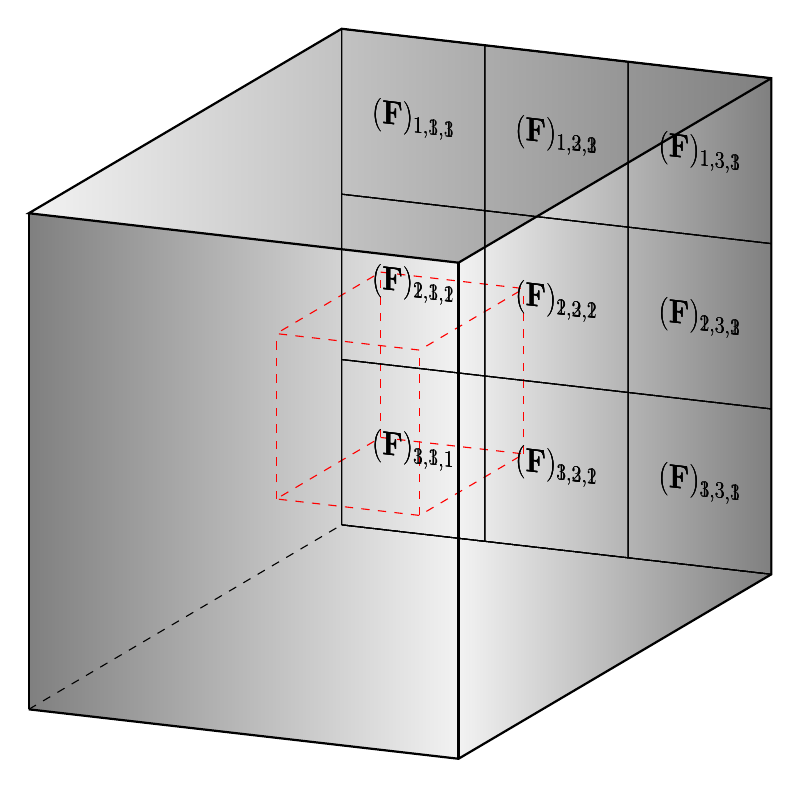
\begin{tikzpicture}[rotate around x = 0,rotate around y=-15, scale=0.7]
  \coordinate (A) at (0,0,9);
  \coordinate (B) at (9,0,9);
  \coordinate (C) at (9,0,0);
  \coordinate (D) at (9,9,0);
  \coordinate (E) at (9,9,9);
  \coordinate (F) at (0,9,9);
  \coordinate (G) at (0,9,0);
  \coordinate (H) at (9,9,0);
  \coordinate (I) at (0,0,0);

  % shading
  \shade[right color=gray!10, left color=black!50] (A) -- (B) -- (E) -- (F) -- cycle;
  \shade[left color=gray!10, right color=black!50] (B) -- (C) -- (D) -- (E) -- cycle;
  \shade[left color=gray!10, right color=black!50] (E) -- (F) -- (G) -- (H) -- cycle;


  % zentralelement
  \draw [dashed, red] (3,6,3) -- ++(3,0,0) -- ++(0,0,3) -- ++(-3,0,0) -- ++(0,0,-3); % top
  \draw [dashed,red] (3,3,3) -- ++(3,0,0) -- ++(0,0,3) -- ++(-3,0,0) -- ++(0,0,-3); % bottom
  \draw [dashed, red] (3,3,3) -- (3,6,3) (3,3,6) -- (3,6,6) (6,3,3) -- (6,6,3) (6,3,6) -- (6,6,6); % connecting
  % \node [red] at (4.5, 4.5, 4.5) {\LARGE $(\ten{F})_C$};

  % borders
  \draw[dashed] (A) -- (I) edge (G) -- (C);
  \draw[thick] (A) -- (B) -- (C) -- (H) -- (G) -- (F) edge (A) -- (E) edge (B) -- (H);


  % front
  \begin{scope}[canvas is plane={O(0,0,9)x(1,0,9)y(0,1,9)},transform shape]
    \foreach \x/\xt in {1.5/1,4.5/2,7.5/3} {
      \foreach \y/\yt in {1.5/3,4.5/2,7.5/1} {
        \coordinate (pos) at (\x,\y);
        \node [] at (pos) {\LARGE $(\ten{F})_{\yt,\xt,1}$};
      }
    }
    \draw[black,step=3] (0,0) grid (9,9);
  \end{scope}

  % right
  \begin{scope}[canvas is plane={O(9,0,9)x(9,0,8)y(9,1,9)},transform shape]
    \foreach \x/\xt in {1.5/1,4.5/2,7.5/3} {
      \foreach \y/\yt in {1.5/3,4.5/2,7.5/1} {
        \coordinate (pos) at (\x,\y);
        \node [] at (pos){\LARGE $(\ten{F})_{\yt,3,\xt}$};
      }
    }
    \draw[black,step=3] (0,0) grid (9,9);
  \end{scope}

  % top
  \begin{scope}[canvas is plane={O(0,9,9)x(1,9,9)y(0,9,8)},transform shape]
    \foreach \x/\xt in {1.5/1,4.5/2,7.5/3} {
      \foreach \y/\yt in {1.5/1,4.5/2,7.5/3} {
        \coordinate (pos) at (\x,\y);
        \node [] at (pos) {\LARGE $(\ten{F})_{1,\xt,\yt}$};
      }
    }
    \draw[black,step=3] (0,0) grid (9,9);
  \end{scope}


\end{tikzpicture}

%%% Local Variables:
%%% mode: latex
%%% TeX-master: "../figs"
%%% End:


\end{document}

%%% Local Variables:
%%% TeX-command-extra-options: "--shell-escape"
%%% TeX-master: "./figs"
%%% End: